\tikzstyle{end} = [circle, minimum size = 0.1cm, draw, inner sep = 0.1pt]
\tikzstyle{leaf} = [circle, minimum size = 0.6cm, draw, inner sep = 0.1pt, blue]
            
\tikzstyle{level 1}=[level distance = 1.5cm, sibling distance = 5cm]
\tikzstyle{level 2}=[sibling distance = 4cm]
\tikzstyle{level 3}=[sibling distance = 1.5cm]
    
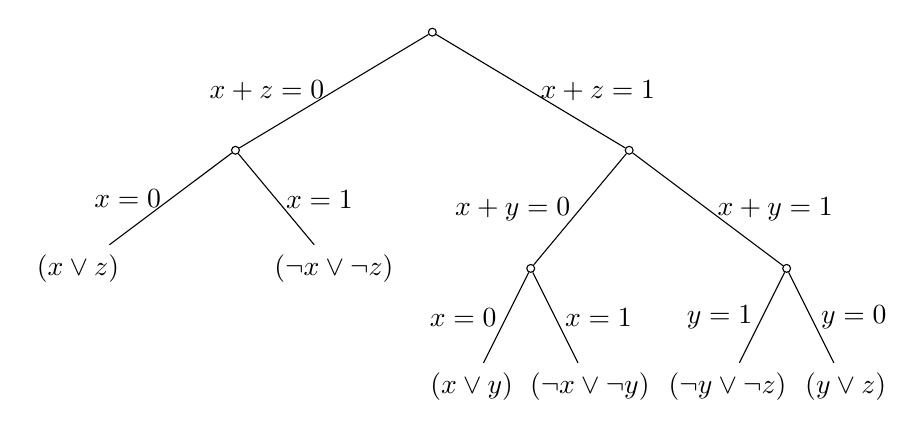
\begin{tikzpicture}[label distance=8mm]
	\node [end] {}
        child {
        	node[end] {}
           	child {
               	node {\alert{$(x \lor z)$}}
                edge from parent
	            node[left] {$x = 0$}
            }
            child[sibling distance = 2.5cm] {
               	node {\alert{$(\neg x \lor \neg z)$}}
                edge from parent
	            node[right] {$x = 1$}
            }
           	edge from parent
            node[left] {$x + z = 0$}
        }
        child {
        	node[end] {}
            child[sibling distance = 2.5cm] {
                node[end] {}
                child {
            		node {\alert{$(x \lor y)$}}
	                edge from parent
    	            node[left] {$x = 0$}
        	    }
                child {
            		node {\alert{$(\neg x  \lor \neg y)$}}
                	edge from parent
	                node[right] {$x = 1$}
    	        }
                edge from parent
                node[left] {$x + y = 0$}
            }
            child {
            	node[end] {}
                child {
            		node {\alert{$(\neg y \lor \neg z)$}}
	                edge from parent
    	            node[left] {$y = 1$}
        	    }
                child {
            		node {\alert{$(y \lor z)$}}
                	edge from parent
	                node[right] {$y = 0$}
    	        }
                edge from parent
                node[right] {$x + y = 1$}
            }
           	edge from parent
            node[right] {$x + z = 1$}
        };
\end{tikzpicture}

%%% Local Variables: 
%%% mode: latex
%%% TeX-master: t
%%% End: 
